\documentclass[12pt]{article}
\usepackage[a4paper,margin=0.75in]{geometry}
\usepackage[utf8]{inputenc}
\usepackage[OT1]{fontenc}
\usepackage[table,usenames,dvipsnames]{xcolor}
\usepackage{array}
\usepackage{varwidth}
\usepackage{tabularx}
\usepackage{amsmath}
\usepackage{hyperref}
\usepackage{enumitem}
\usepackage{graphicx}
\usepackage{tcolorbox}
\usepackage{forest}
\usepackage{parskip}
\renewcommand*\familydefault{\sfdefault}

% from https://gist.github.com/nhtranngoc/88b72d9bfb656a3de227eea38ed80627
\usepackage{listings}
% \usepackage{fontspec}
% \setmonofont{Consolas}

\definecolor{background}{RGB}{39, 40, 34}
\definecolor{string}{RGB}{230, 219, 116}
\definecolor{comment}{RGB}{117, 113, 94}
\definecolor{normal}{RGB}{248, 248, 242}
\definecolor{identifier}{RGB}{166, 226, 46}

\lstset{
  % language=c,                			% choose the language of the code
  numbers=left,                   		% where to put the line-numbers
  stepnumber=1,                   		% the step between two line-numbers.        
  numbersep=5pt,                  		% how far the line-numbers are from the code
  numberstyle=\scriptsize\color{black}\ttfamily,
  backgroundcolor=\color{background},  		% choose the background color. You must add \usepackage{color}
  showspaces=false,               		% show spaces adding particular underscores
  showstringspaces=false,         		% underline spaces within strings
  showtabs=false,                 		% show tabs within strings adding particular underscores
  tabsize=4,                      		% sets default tabsize to 2 spaces
  captionpos=b,                   		% sets the caption-position to bottom
  breaklines=true,                		% sets automatic line breaking
  breakatwhitespace=true,         		% sets if automatic breaks should only happen at whitespace
  title=\lstname,                 		% show the filename of files included with \lstinputlisting;
  basicstyle=\color{normal}\ttfamily\footnotesize,	    	% sets font style for the code
  keywordstyle=\color{magenta}\ttfamily,	% sets color for keywords
  stringstyle=\color{string}\ttfamily,		% sets color for strings
  commentstyle=\color{comment}\ttfamily,	% sets color for comments
  emph={format_string, eff_ana_bf, permute, eff_ana_btr},
  emphstyle=\color{identifier}\ttfamily
}

\newtcolorbox{mybox}[3][]
{
  colframe = #2!25,
  colback  = #2!10,
  coltitle = #2!20!black,  
  title    = {#3},
  #1,
}

\hypersetup{
    colorlinks=true,
    linkcolor=blue,
    filecolor=magenta,      
    urlcolor=cyan,
    pdftitle={Overleaf Example},
    pdfpagemode=FullScreen,
}

\title{\textbf{COL331 Assignment 2: Hard Track}}
\author{Aniruddha Deb \\ \texttt{2020CS10869}}
\date{April 2023}

\begin{document}

\maketitle

\section{Deadline Monotonic and Rate Monotonic Scheduling}

Implementing a sched class from scratch for deadline monotonic scheduling was
infeasible, and hence we use a kthread-based scheduling algorithm implemented
on top of the linux real-time fifo scheduler. The scheduler uses a linked list 
of tasks sorted in decreasing order of priority along with a dispatcher thread 
to schedule tasks whenever they are registered/yielded.

The main process control block structure that we use is built upon the linux 
task\_struct, with additional fields.

\begin{lstlisting}[language=C]
struct dm_pcb {
 	struct list_head list_node;
	struct list_head wait_queue_node;
	struct task_struct* linux_task;
	struct hrtimer timer;
	unsigned int period;
	unsigned int deadline;
	unsigned int duration;
	unsigned int state;

	// negative of deadline
	int priority;
	// used to tiebreak between tasks with the same priority
	int priority_epsilon;

	struct sched_param old_sched_params;
};
\end{lstlisting}

Here:
\begin{itemize}
    \item period, deadline and duration store the task's period, deadline and 
        duration as specified in the syscall
    \item state stores the current state of the task: one of running, sleeping
        or ready
    \item priority and priority\_epsilon are used to determine the task's 
        priority. priority\_epsilon is zero for all tasks who have not allocated
        resources, and is only used while tiebreaking between tasks by the 
        scheduler when priority inheritance happens.
\end{itemize}

\subsection{registering and deregistering}

One common function, \texttt{\_\_register\_dm} is used to register both deadline
monotonic and rate monotonic tasks. Rate monotonic tasks are built upon
Deadline monotonic tasks, and use the same scheduler and task queue, with the
only difference being that the deadline and period are the same for these tasks.

For the schedulability check, we implement the algorithm in [1]: this is a 
neccessary and sufficient check for checking whether a given set of tasks is 
deadline schedulable, and this was tested with testcases where tasks had both 
same and different periods.

To register a task, it's PCB is initialized and it is inserted into the list at 
an appropriate position. The schedulability check is then run: if it fails, the
task is removed. If not, a timer is registered with the task which triggers 
a scheduling callback with a frequency equal to the period of the task. This 
scheduling callback sets the task state to ready, and wakes up the dispatcher 
kernel thread to update the currently running task.

To deregister a task, the task is removed from the task list, and it's original
CFS priority is restored. It's PCB is deleted, and any resources that it 
acquired are relinquished.

\subsection{yield}

The yield call sets the state of the process to sleeping and the currently running
task to NULL. It then wakes up the dispatcher thread to reschedule the tasks.

\subsection{Additional implementation details}

Poor accuracy was observed with using a \texttt{timer\_list}, so a \texttt{hrtimer}
was used instead.

\pagebreak
\section{Priority Ceiling Protocol}

The priority ceiling protocol was described in [2], and is implemented according
to the following flowchart:

\begin{figure}[!htbp]
    \centering
    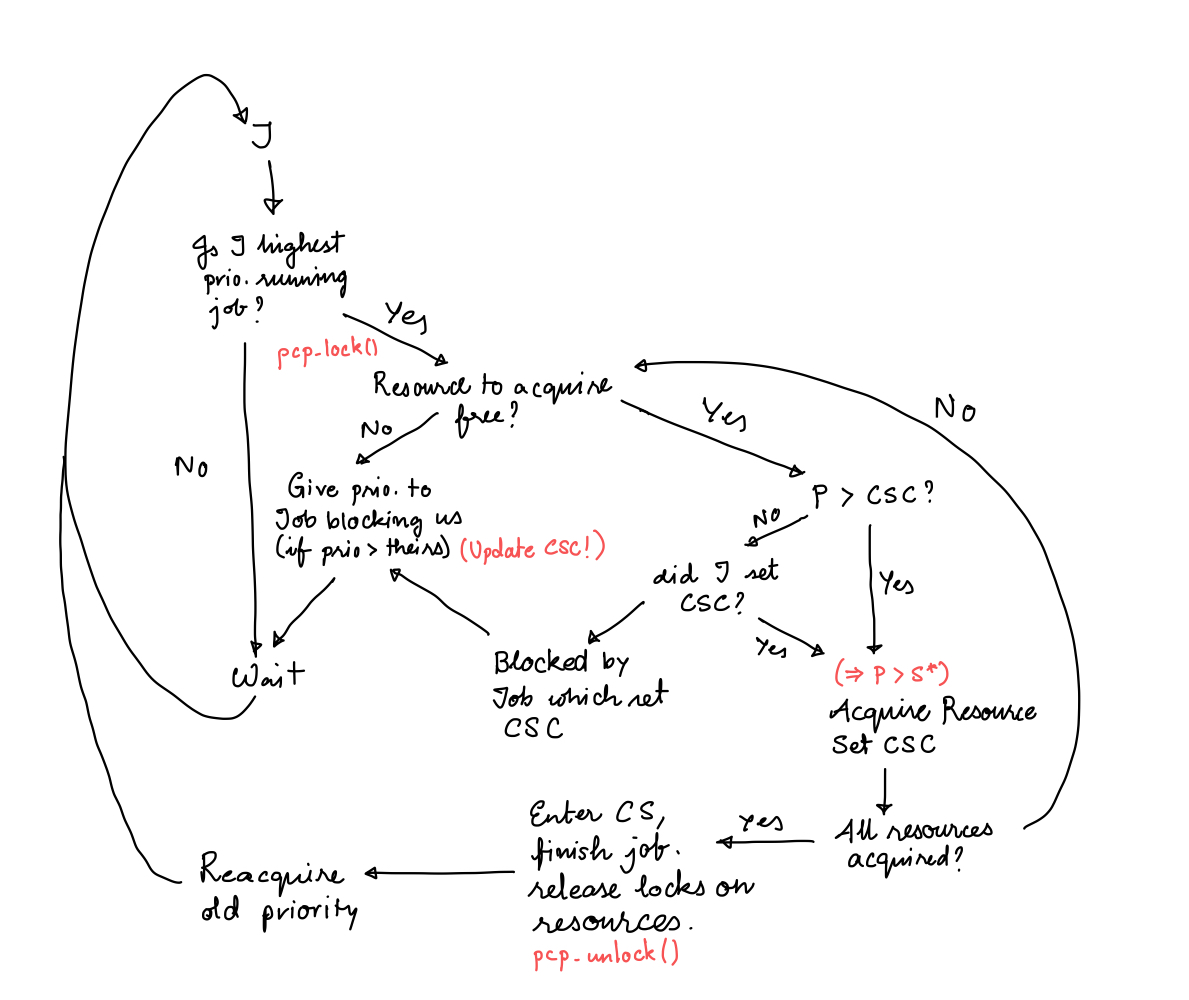
\includegraphics[width=0.9\textwidth]{pcp.jpeg}
\end{figure}

We assume a fixed set of resources (10), all of which have the following 
structure:

\begin{lstlisting}[language=C]
struct resource_t {
	struct mutex mtx;
	int wait_queue_len;
	struct list_head wait_queue;
	int rid;
	int ceiling;

	struct dm_pcb* owner;
	int owner_priority_before_acquisition;
	int owner_priority_epsilon_before_acquisition;
};
\end{lstlisting}

The fields are self-explanatory. The \texttt{owner\_priority\_before\_acquisition} fields 
store the priority the task had before acquiring the resource, so that we can 
invert the priority once the task is done using the resource and leaves it's 
critical section.

\subsection{Changes to vanilla DM scheduling}

Priority inheritance required adding the epsilon term to the priority class:
since we're relying on the dispatcher to schedule our threads, if a task A with
a high deadline has acquired a resource and a task B with a low deadline is 
waiting on it, then A acquires B's priority (deadline). Now, the task scheduler 
needs a way to schedule A before B everytime, even if A is after B in the queue.
We cannot add an epsilon to A's priority, as it is an integer and may clash with
some other priority. Hence, we use another field for storing the epsilon, and
compare this value if the two priorities of tasks are equal while scheduling.

A simpler way to do this would have been to set priority = -deadline*64, and this 
would support an epsilon of 0 to 63 (basically treat priority as a fixed point number. 
However, having a separate field supports a larger number of overlapping tasks.

\subsection{Resource mapping and starting PCP}

The resource map syscall is used to determine the priority ceiling of a resource.
The priority ceiling is defined as the maximum priority of any job that may
acquire the resource while it is running. To compute this, we need to know the 
set of jobs that will acquire that resource beforehand. This information is 
provided using this method.

The start PCP syscall is used to initialize the resources' locks and lists and 
set the timers of all the tasks that take part in PCP.

\subsection{Locking and Unlocking}

Most of the logic of PCP lies in locking and unlocking, and these two algorithms
are implemented according to the above flowchart.

We may be blocked when we try to lock (acquire) a resource in two cases:
\begin{enumerate}
    \item The resource is in use by another job J. We are then blocked by job J,
       and we transfer our priority to J if it's greater than J's current priority.
   \item The resource is free, but we are under the current system ceiling (and 
       neither have we set the current system ceiling). In this case, we are 
       blocked by the job that set the current system ceiling. We can't transfer 
       our priority as it would anyway be less than (or equal to) the job
       that set the current system ceiling, so we transfer one epsilon to it 
       (if our priority is equal to it) so that it may be scheduled always.
\end{enumerate}

If we are blocked, we register ourselves in the waitqueue in order, go to sleep by 
sending a SIGSTOP and calling the scheduler to reschedule. If not, we can 
acquire the resource (after setting the old priority fields in the resource 
appropriately) and continue executing.

For unlocking a resource, we first update the resource statistics, get back to 
our old priority before acquiring the resource and then unlock the mutex. We 
then choose the first element in the wait queue (this has the highest priority
among the waiting processes), and assign the resource to it. Since only one 
task can run at any time and we have just stopped running after releasing this 
resource, either we hold more resources and will continue to run or this new 
task will run. We let the scheduler decide this: the new task will be scheduled
after being given this resource. If it fails to acquire any other resource it 
needs which we hold, it would be blocked and we will be rescheduled by the 
scheduler in the other program's PCP lock syscall.

\section{References}

\begin{enumerate}
    \item Audsley, Neil C., et al. "Deadline monotonic scheduling." (1990).
    \item Sha, L., et al. “Priority Inheritance Protocols: An Approach to Real-Time Synchronization.” IEEE Transactions on Computers, vol. 39, no. 9, Sept. 1990, pp. 1175–85. DOI.org (Crossref), https://doi.org/10.1109/12.57058.
\end{enumerate}

\end{document}
